\documentclass{article}

\usepackage{booktabs} 
\usepackage[english]{babel}
\usepackage{graphicx}
\usepackage{amsmath}
\usepackage{listings}
\usepackage{url}

\title {Project Report}
\date{21 December 2016}
\author{Elise Mol, Wendy Nieuwkamer, and Isobel Smith}

\begin{document}

\maketitle

\section{Problem}
	
	After three months of learning about several machine learning techniques and classifying algorithms it was time to put our newly gained skills into practice. We decided to try our hand at one of the competitions hosted by Kaggle. The challenge we chose is Leaf Classification; the objective of the competition is to use binary leaf images and their extracted features to predict what species each leaf belongs to. The dataset which was provided includes around 1584 images of leaf specimens; these samples include 99 species. From every image three sets of features are extracted: a shape contiguous descriptor, an interior texture histogram and a fine-scale margin histogram. Every feature is represented as a 64-attribute vector. 
	
	As the competition started at 30 August 2016, there were already quite some submissions made and kernels active. One of them stood out, namely "10 Classifier Showdown in Scikit-Learn". In this kernel Jeff Delaney compared ten classifiers which are part of the python library Scikit-Learn. The results of his experiment are shown in figure \ref{fig:showdown}. In his experiment Delaney used the default setup for the classifiers , combined with semi-random parameters. He notes that the performance of the classifiers could be improved by tuning the hyper-parameters. Thus, our research question is whether we can improve the accuracy found by Delaney by tuning the hyper-parameters of the classifiers.
	
	\begin{figure} 
		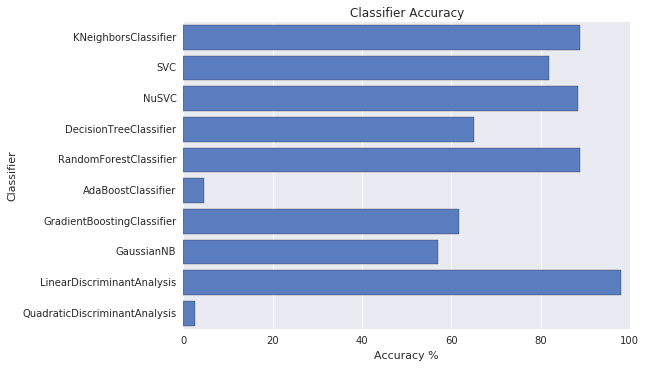
\includegraphics[width=\linewidth]{results-showdown.png}
		\caption{The 10 Classifier Showdown}
		\label{fig:showdown}
	\end{figure}
	
	As we did not have time to run experiments for all ten classifiers, we decided to look into five of them. We chose the K-neigbors classifier, decision tree classifier and Gaussian Naive Bayes as they had relatively decent accuracy at respectively 88\%, 65\%, and 57\%. Also, we had some background in these algorithms as they had been taught in our Machine Learning course. Additionally, we decided to choose either Ada boost or quadratic discriminant analysis as they could improve the most with found accuracies of 4.5\% and 2.5\%. 

\newpage
\section{The algorithms}
	Before we could start optimizing the hyper-parameters we had to research the algorithms we chose. In order to discover the most relevant information for our experiment we aimed to answer the following questions:
	
	\begin{itemize}
		\item How does the classifier work? 
		\item Which hyper-parameters exist for each classifier??
		\item Which hyper-parameters have the most effect on the classifier?
	\end{itemize}
	
	The answers to these questions are specific to the Scikit-Learn package.
	
	\subsection{K-neighbors}
		The k-neighbors algorithm classifies an object according to the k nearest objects from the training set. For a higher k noise might be filtered out, but class boundaries might become more vague and less accurate. Thus, it would be interesting to find out which value of k gives the highest accuracy for our dataset. There are two ways of computing the class from the neigbors. The first one is by giving all the neighbors equal weight, no matter how far or close they are.  The second is to give each neighbor a weight relative to its distance. The weighted version of the algorithm is especially useful when a dataset has areas with a varying density of training examples. 
	
	\subsection{Decision Tree Classifier}
	
	\subsection{Gaussian Naive Bayes}
	
	\subsection{Ada Boost Classifier}
	
	\subsection{Quadratic Discriminant Analysis}

\section{Choices made and justifications}
	Which classifiers you chose ; why?  
	Describe the relevant features of the classifiers.

\newpage
\section{Hyper-parameter optimization}

	Hyper-parameter optimization is one of the most important steps in machine learning \cite{bardenet}. The goal is to find the best hyper-parameters for the given classifier, in order to minimize the loss function and to avoid over-fitting \cite{Bergstra}. Some hyper-parameter optimization algorithms do not only find the best hyper-parameters, but identify those that carry the most weight \cite{Bergstra}.
	There are two hyper-parameter optimization algorithms built into Scikit-Learn: grid search and randomized parameter optimization \cite{gridsearch}. Scikit-Learn also provides alternative methods such as model specific cross validation  \cite{HyperparameterOptimisationWiki}, but we did not use those.  
	
	\subsection{Grid Search}
	
		Grid Search optimizes hyper-parameters by iterating over all of the variables in a given range and selecting the best combination to use in the chosen classifier. Grid search is guided by a performance metric, such as classification accuracy, which is usually measured by cross-validation \cite{HyperparameterOptimisationWiki}. A disadvantage of grid search is that it can be time consuming and computationally expensive to run, \cite{HyperparameterOptimisationWiki}.

		As grid search was recommended to us by our teacher Rein van den Boomgaard, and is the widely used to optimize hyper-parameters, we decided to use it in our project.
The use of Grid Search was easy as Scikit-Learn has a built-in class called GridSearchCV \cite{gridsearch}, which is defined below:
		
		
	\begin{lstlisting}
GridSearchCV(estimator, param_grid, scoring=None, fit_params=None, 
   n_jobs=1, iid=True, refit=True, cv=None, verbose=0, 
   pre_dispatch='2*n_jobs', error_score='raise',
   return_train_score=True)
	\end{lstlisting}
		
	When an instance of GridSearch is initialized, it takes an estimator, a param\textunderscore grid and any other parameters. The estimator would be our classification functions KNeighborsClassifier, DecisionTreeClassifier, and AdaBoostClassifier. The param\textunderscore grid is a dictionary with the parameters you want to optimize as the keys, and the range of parameters to try as the values. The grid search algorithm will then run the given classifier over the entire parameter grid in order to find the best possible combination. We also chose to use 5-fold cross validation instead of the default 3-fold cross validation by passing cv=5 to GridSearchCV.

	\subsection{Implementation}
		


		We used the built-in grid search function from scikit-learn, and ran it on each of our classifiers. The range of values selected for the hyperparameters were chosen through trial and error. We set $cv=5$, as we decided to use 5 folds in the KFold cross validation scheme. 


		
		The output of GridSearch is the a dict, with the names of the hyperparameter as keys, and the optimal result as values. 
		
		\begin{lstlisting}
{hyperparameter: optimal value, hyperparameter: optimal value}
		\end{lstlisting}

	We than ran the classifiers on the training data with the optimal parameters, and computed the new accuracy scores. 





\section{Results}

The accuracy of classifiers with optimised hyperparameters were graphed against those without optimised hyperparameters:

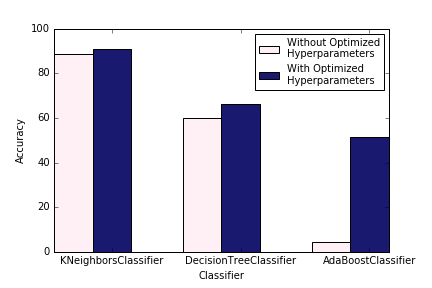
\includegraphics[scale=0.7]{acc_class}

In each of the cases, grid search clearly improved the accuracy of the classifier, reaffirming the importance of hyperparameter optimisation in machine learning. 

AdaBoost was significantly improved by hyperparameter optimisation, from $4.56\%$ to $51.52\%$. This is due to the fact that the default parameters that were used in the 10 Classifier Showdown \cite{showdown} were inadequate for the leaf classification problem. K-neighbors was improved from $88.89\%$ to $90.91\%$, and Decision Trees were improved from $60.10\%$ to $66.16\%$. 

\subsection{AdaBoost}

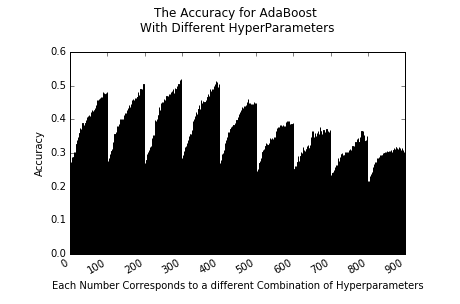
\includegraphics[scale=0.6]{adaboost_crop}

The graph above shows how grid search across each of the different hyperparameter combinations improved the accuracy of AdaBoost. The numbers on the x-axis corresponds to a different combination of hyperparameters. As can be clearly seen from the graph the amount of possible combinations was very high. This was computationally quite expensive, and running grid search on AdaBoost took a long time compared to the other classifiers. 

The optimal hyperparameters for AdaBoost were found to be $n$\textunderscore $estimators = 72$ with $learning$ \textunderscore $rate = 0.03$

\subsection{Decision Trees}


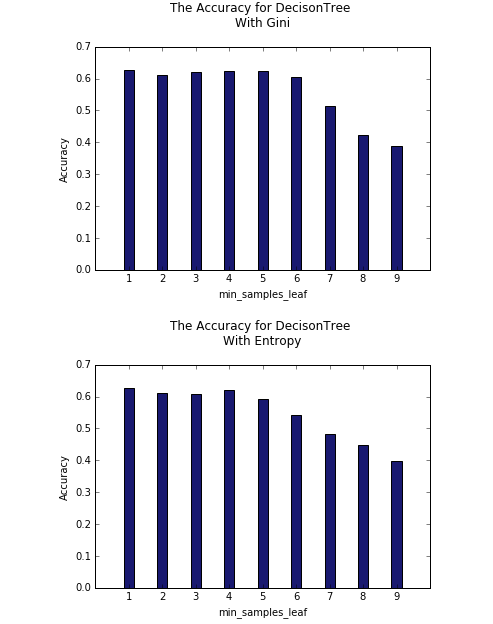
\includegraphics[scale=0.6]{d_trees_crop}

The accuracy of decision trees were comparatively not as improved as much as the accuracy of the other two were. This was because the default parameters used in the 10 classifier showdown \cite{showdown} happened to be similar to the optimal parameters as found by grid search. 

Interestingly, the difference between grid search using entropy, or using Gini was minimal, as can be seen from the graph. This suggests that for this problem the splitting criteria hyperparameter does not hold much weight as other hyperparameters might. 

The optimal hyperparameters found for decision trees were to be $splitter = 'best', criterion = 'entropy'$ and $min$ \textunderscore $samples$ \textunderscore $leaf = '1'$

\subsection{K-Neighbors}

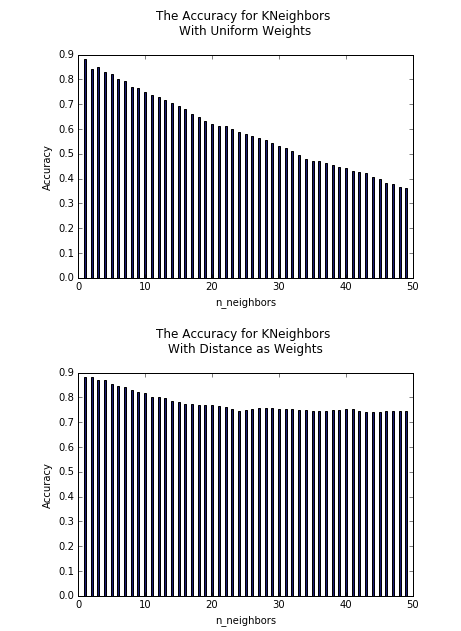
\includegraphics[scale=0.6]{k-nboors}

One of the hyperparameters we needed to tune for k-neighbors were the wieights. We needed to choose between using uniform weights or distance as weights. The accuracy graphs clearly show that the accuracy rate for k-neighbors with uniform weights quickly tails of when the number of neighbors increases, whereas the accuracy when using distance as weights remains relatively high as the number of neighbours increases. 

The optimal hyperparameters chosen for K-Neighbors was that $n$ \textunderscore $neighbors = 1,$ and $weights = 'uniform'$


\section{Evaluation of Approach and Solution} 
	All the curves, the results


	The other hyperparamter optimisation function built in to  scikit-learn is randomized parameter optimisation \cite{gridsearch}. Instead of iterating over each potential combination of parameters, like grid search, it randomly selects these combinations. The advantage if this is that it can be less computationally expensive than grid search, and that adding parameters that do not influence the performance does not decrease the algorithms efficiency. The number of random samples that are tried can be specified.  As AdaBoost had such a high amount of hyperparameter combinations, using randomised parameter optimisation in this case may reduced the computation time. 

	An improvement would be a better way to select the range of hyperparameters to test, rather than to use trial and error.

	Another improvement would be to look at choosing another value for the k-folds, instead of default 5. 

\bibliographystyle{unsrt}
\bibliography{ProjectReport}




















\end{document}
